%1_probability.tex
%notes for the course Probability and Statistics COMS10011 
%taught at the University of Bristol
%2018_19 Conor Houghton conor.houghton@bristol.ac.uk

%To the extent possible under law, the author has dedicated all copyright 
%and related and neighboring rights to these notes to the public domain 
%worldwide. These notes are distributed without any warranty. 

\documentclass[11pt,a4paper]{scrartcl}
\typearea{12}
\usepackage{graphicx}
%\usepackage{pstricks}
\usepackage{listings}
\usepackage{color}
\lstset{language=C}
\usepackage{fancyhdr}
\pagestyle{fancy}
\lfoot{\texttt{github.com/COMS10011/2018\_19}}
\lhead{COMS10007 1\_probability - Conor}
\begin{document}

\section*{Introduction}

In probability and statistics we develop the tools for studying data
that is uncertain or noisy and processes that have a random
element. Probability and statistics is important to computer
scientists of all types; some computer scientists use computers to
manipulate data, or to make statistical inferences about data in, for
example, machine learning, other computer scientists make products
that need to be tested and statistics is needed to interpret the
results of user testing.

Imaging a gambler wants to decide if a coin is fair; imagine they toss
it five times and get a head each time. Can they decide that the coin is
fair. It is clear that they can't say that it is
impossible that a fair coin would turn up heads five times; it is just
pretty unlikely. They could say that there is only a one in
\begin{equation}
2^{5}=32
\end{equation}
chance that a fair coin would produce that result. Since
$(1-1/32)*100\approx 97$ it would seem that gambler could be $97\%$
certain the coin was unfair. This isn't the end of the story though:
five harps would have been equally suprising; so perhaps the thing to
say is that there is only a one in
\begin{equation}
2^{4}=16
\end{equation}
the coin would produce such an unlikely result. Does this means the
gambler can only be $94\%$ certain the coin is unfair? The idea of
this unit it to learn how to calculate probabilities, the probability
of five heads is an easy example of this, and how to make inferences,
such as deciding the chance the coin is unfair.


%% change to 1 9 90 900 etc
It is very easy to confuse yourself with probability; here is a
confusing problem. An evil genius has decided to tattoo their names on
some peoples foreheads and in the usual over-elaborate evil genius
manner they do it according to a diabolic game. A person is selected
and forced into the tattoo parlour, the evil genius rolls two die and
if they show two sixes, they tattoo the person and the game ends,
otherwise the lucky person is released and the evil genius selects
nine new people. Again, the evil genius rolls the die, again, if it
gives two sixes then they tattoo everyone and the game ends, if not,
they let them leave, select 90 people and roll the die. The process
repeats, multiplying the number each time by ten, until the dice comes
up with two sixes, the people in the parlour are tattooed and the game
ends. If you are forced into the perilous parlour, what is the chance you'll
end up with a tattoo on your forehead. Is it the relatively modest one
in 36, or, given that 90\% of people who enter the room end up
tattooed, is it nine in ten?

This is a problem for you to think about yourselves, the point is that
in statistics and probability it isn't enough to be good at
calculating probabilities, though this is useful, it is important to
know what you are trying to calculate. To avoid getting confused we
need some notation and some mathematical machinery and that's what we
are going to do now.

\section*{1: Probability}

To start with we need to terminology and notation and this begins with
a \textbf{sample space} $X$, this is the set of points; the idea is
that these points are the possible outcomes of an experiment, or, it
is said, the outcome of a \textbf{trial}. Initially it is useful to
think of discrete sample spaces with individual points, for example,
for the coin where the experiment is tossing it once, the sample space
has two points:
\begin{equation}
S=\{H,T\}
\end{equation}
where the two points $H$ and $T$ correspond to heads and harps, the
two possible outcomes of flipping the coin. If the experiment is
tossing the coin twice then the sample space has four points:
\begin{equation}
S=\{HH,HT,TH,TT\}
\end{equation}
unless the outcome of a trial only records the number of heads and
harps, not the order, in which case the sample space has three points:
\begin{equation}
S=\{HH,HT,TT\}
\end{equation}
which $HT$ stand for heads then harps as well as harps then
heads. Later we will look at continuous sample spaces where the
experiment takes a value in a continuum, so we could have, for example
\begin{equation}
\mathcal{L}=[0,\infty)
\end{equation}
as the sample space for the experiment of measuring the length of a
song on the radio.

An \textbf{event} in a discrete sample space $X$ is a subset $E\subset
X$. If the sample space was $\{1,2,3,4,5,6\}$ corresponding to the
face values of a dice, then the set of even sides $\{2,4,6\}$ is an
example event. This is a useful notation because we might want to
calculate the probability for an event as well as for the individual
points; we might wonder, what is the chance the dice will show an even
value, that is, what is the chance the outcome is an element of the
event.

Now, we want to define a \textbf{probability} on a sample space
$X$. Obviously a probability is the chance of something happening, but
before doing that part, we need to look at some of the properties that
a probability needs to have. Formally, a probability is a map $P$ from
events to real numbers such that
\begin{enumerate}
\item $P(A)\ge 0$ for all events.
\item $P(X)=1$
\item If $A\cap B=\emptyset$ for two events $A$ and $B$ then 
\begin{equation}
P(A\cup B)=P(A)+P(B)
\end{equation}
\end{enumerate}
where $A\cap B$ and $A\cup B$ are the intersection and union of $A$
and $B$ and $\emptyset$ is the empty set. This lists the properties we
expect a probability to have; the key thing being if two events are
disjoint then the probability of the joint event is the sum of the
probabilities of the individual events. For example the probability of
getting one or two on a dice is a third, the probability of getting a
three is a sixth; putting these together, the probablity of getting a
one, two or three is a half.

\section{Counting things}

The is a class of problems where calculating probabilities can be
reduced to counting things; this basically works using the rule above
that says $P(A\cup B)=P(A)+P(B)$ if $A\cap B=\emptyset$. If, for
example, all the points in a sample space have the same probability, say $q$, then
this rule means that the probability of an event is is 
\begin{equation}
p(A)=(\mbox{number of points in }A)\times q
\end{equation}
From the rule $P(X)=1$ it also follows that 
\begin{equation}
q=1/(\mbox{total number of points in the sample space})
\end{equation}
Incidentally, a few different notations are used for the number of points in a set, I will use
\begin{equation}
\#(A):=\mbox{number of points in }A
\end{equation}
where \lq{}$:=$\rq{} means \lq{}is defined as\rq{} or \lq{}is used to
mean\rq{}. Another common notation is
\begin{equation}
|A|:=\mbox{number of points in }A
\end{equation}

One standard example for calculating probabilities is the problem of
working out the probability of getting different card hands in poker;
for definiteness lets consider five card stud poker where the player
is dealt five card. A pair is the hand where two cards are the
same and all the rest of different. What is the probability of getting a pair. The total number
of different hands in poker is 52 choose five:
\begin{equation}
\left(\begin{array}{c}52\\5\end{array}\right)=\frac{52\times 51\times 50\times 49\time 48}{1\times 2 \times 3 \times 4\times 5}=2598960
\end{equation}
where the binomial coefficient
\begin{equation}
\left(\begin{array}{c}n\\r\end{array}\right)=\frac{n!}{r!(n-r)!}
\end{equation}
counts the number of subsets of size $r$ in a set of $n$ objects and 
\begin{equation}
n!=n\times (n-1)\times (n-2)\times \ldots \times 2 \times 1
\end{equation}
How many pairs are there; well there are 13 possible values for the
pair in two suits out of four, giving six possible pairs of suits,
there are 12 choose three ways of picking out the other three values,
there is no constraint on the suit of the non-pair cards, giving
\begin{equation}
\#(\mbox{set of pairs})=13\times 6\times \frac{12\times 11\times 10}{6}\times 4^3=1098240
\end{equation}
Thus
\begin{equation}
p(\mbox{pair})=\frac{1098240}{2598960}\approx 0.42
\end{equation}

A classic problem is the birthday party problem; a common intuition is
that it is very rare to find people in a group with the same birthday;
it isn't the case: in a group of 23 people there is a one in two
chance that two with share a birthday. Roughly speaking the point is that
there are lots of pairs of people. Now, lets ignore leap years and the
impact the long long nights of January have on the birth rate in
September. So, say there are 20 people in a
group, a point in the sample space is a list of 20 birthdays. The
number of possible lists, and hence the size of the sample space is
$365^{20}$. However, the number of lists where all the birthdays are
different is
\begin{equation}
\#(\mbox{lists with different birthdays})=365\times 364 \times \ldots \times 347 \times 346
\end{equation}
This means the probability no pair has a shared birthday is
\begin{equation}
p(\mbox{no shared birthday})=\frac{365}{365}\frac{364}{365}\ldots\frac{347}{365}\frac{346}{365}\approx 0.5886
\end{equation}
and hence
\begin{equation}
p(\mbox{at least one shared birthday})=1-p(\mbox{no shared birthday})\approx 0.414
\end{equation}
Put another way, the probability of a shared birthday in a group of $n$ people is
\begin{equation}
p(\mbox{at least one shared birthday},n)=1-\prod_{i=0}^{n-1}\frac{365-i}{365}
\end{equation}
where the big pi symbol is the produce symbol, list the big sigma used
for summing but for products. The probability graph can be seen in Fig.~\ref{fig_birthday}.


\begin{figure}[thb]
\begin{center}
% GNUPLOT: LaTeX picture with Postscript
\begingroup
  \makeatletter
  \providecommand\color[2][]{%
    \GenericError{(gnuplot) \space\space\space\@spaces}{%
      Package color not loaded in conjunction with
      terminal option `colourtext'%
    }{See the gnuplot documentation for explanation.%
    }{Either use 'blacktext' in gnuplot or load the package
      color.sty in LaTeX.}%
    \renewcommand\color[2][]{}%
  }%
  \providecommand\includegraphics[2][]{%
    \GenericError{(gnuplot) \space\space\space\@spaces}{%
      Package graphicx or graphics not loaded%
    }{See the gnuplot documentation for explanation.%
    }{The gnuplot epslatex terminal needs graphicx.sty or graphics.sty.}%
    \renewcommand\includegraphics[2][]{}%
  }%
  \providecommand\rotatebox[2]{#2}%
  \@ifundefined{ifGPcolor}{%
    \newif\ifGPcolor
    \GPcolorfalse
  }{}%
  \@ifundefined{ifGPblacktext}{%
    \newif\ifGPblacktext
    \GPblacktexttrue
  }{}%
  % define a \g@addto@macro without @ in the name:
  \let\gplgaddtomacro\g@addto@macro
  % define empty templates for all commands taking text:
  \gdef\gplbacktext{}%
  \gdef\gplfronttext{}%
  \makeatother
  \ifGPblacktext
    % no textcolor at all
    \def\colorrgb#1{}%
    \def\colorgray#1{}%
  \else
    % gray or color?
    \ifGPcolor
      \def\colorrgb#1{\color[rgb]{#1}}%
      \def\colorgray#1{\color[gray]{#1}}%
      \expandafter\def\csname LTw\endcsname{\color{white}}%
      \expandafter\def\csname LTb\endcsname{\color{black}}%
      \expandafter\def\csname LTa\endcsname{\color{black}}%
      \expandafter\def\csname LT0\endcsname{\color[rgb]{1,0,0}}%
      \expandafter\def\csname LT1\endcsname{\color[rgb]{0,1,0}}%
      \expandafter\def\csname LT2\endcsname{\color[rgb]{0,0,1}}%
      \expandafter\def\csname LT3\endcsname{\color[rgb]{1,0,1}}%
      \expandafter\def\csname LT4\endcsname{\color[rgb]{0,1,1}}%
      \expandafter\def\csname LT5\endcsname{\color[rgb]{1,1,0}}%
      \expandafter\def\csname LT6\endcsname{\color[rgb]{0,0,0}}%
      \expandafter\def\csname LT7\endcsname{\color[rgb]{1,0.3,0}}%
      \expandafter\def\csname LT8\endcsname{\color[rgb]{0.5,0.5,0.5}}%
    \else
      % gray
      \def\colorrgb#1{\color{black}}%
      \def\colorgray#1{\color[gray]{#1}}%
      \expandafter\def\csname LTw\endcsname{\color{white}}%
      \expandafter\def\csname LTb\endcsname{\color{black}}%
      \expandafter\def\csname LTa\endcsname{\color{black}}%
      \expandafter\def\csname LT0\endcsname{\color{black}}%
      \expandafter\def\csname LT1\endcsname{\color{black}}%
      \expandafter\def\csname LT2\endcsname{\color{black}}%
      \expandafter\def\csname LT3\endcsname{\color{black}}%
      \expandafter\def\csname LT4\endcsname{\color{black}}%
      \expandafter\def\csname LT5\endcsname{\color{black}}%
      \expandafter\def\csname LT6\endcsname{\color{black}}%
      \expandafter\def\csname LT7\endcsname{\color{black}}%
      \expandafter\def\csname LT8\endcsname{\color{black}}%
    \fi
  \fi
  \setlength{\unitlength}{0.0500bp}%
  \begin{picture}(5040.00,3528.00)%
    \gplgaddtomacro\gplbacktext{%
      \csname LTb\endcsname%
      \put(946,704){\makebox(0,0)[r]{\strut{} 0}}%
      \put(946,1211){\makebox(0,0)[r]{\strut{} 0.2}}%
      \put(946,1718){\makebox(0,0)[r]{\strut{} 0.4}}%
      \put(946,2224){\makebox(0,0)[r]{\strut{} 0.6}}%
      \put(946,2731){\makebox(0,0)[r]{\strut{} 0.8}}%
      \put(946,3238){\makebox(0,0)[r]{\strut{} 1}}%
      \put(1078,484){\makebox(0,0){\strut{} 0}}%
      \put(1969,484){\makebox(0,0){\strut{} 15}}%
      \put(2861,484){\makebox(0,0){\strut{} 30}}%
      \put(3752,484){\makebox(0,0){\strut{} 45}}%
      \put(4643,484){\makebox(0,0){\strut{} 60}}%
      \put(176,1983){\rotatebox{-270}{\makebox(0,0){\strut{}probability of a match}}}%
      \put(2860,154){\makebox(0,0){\strut{}size of group}}%
    }%
    \gplgaddtomacro\gplfronttext{%
    }%
    \gplbacktext
    \put(0,0){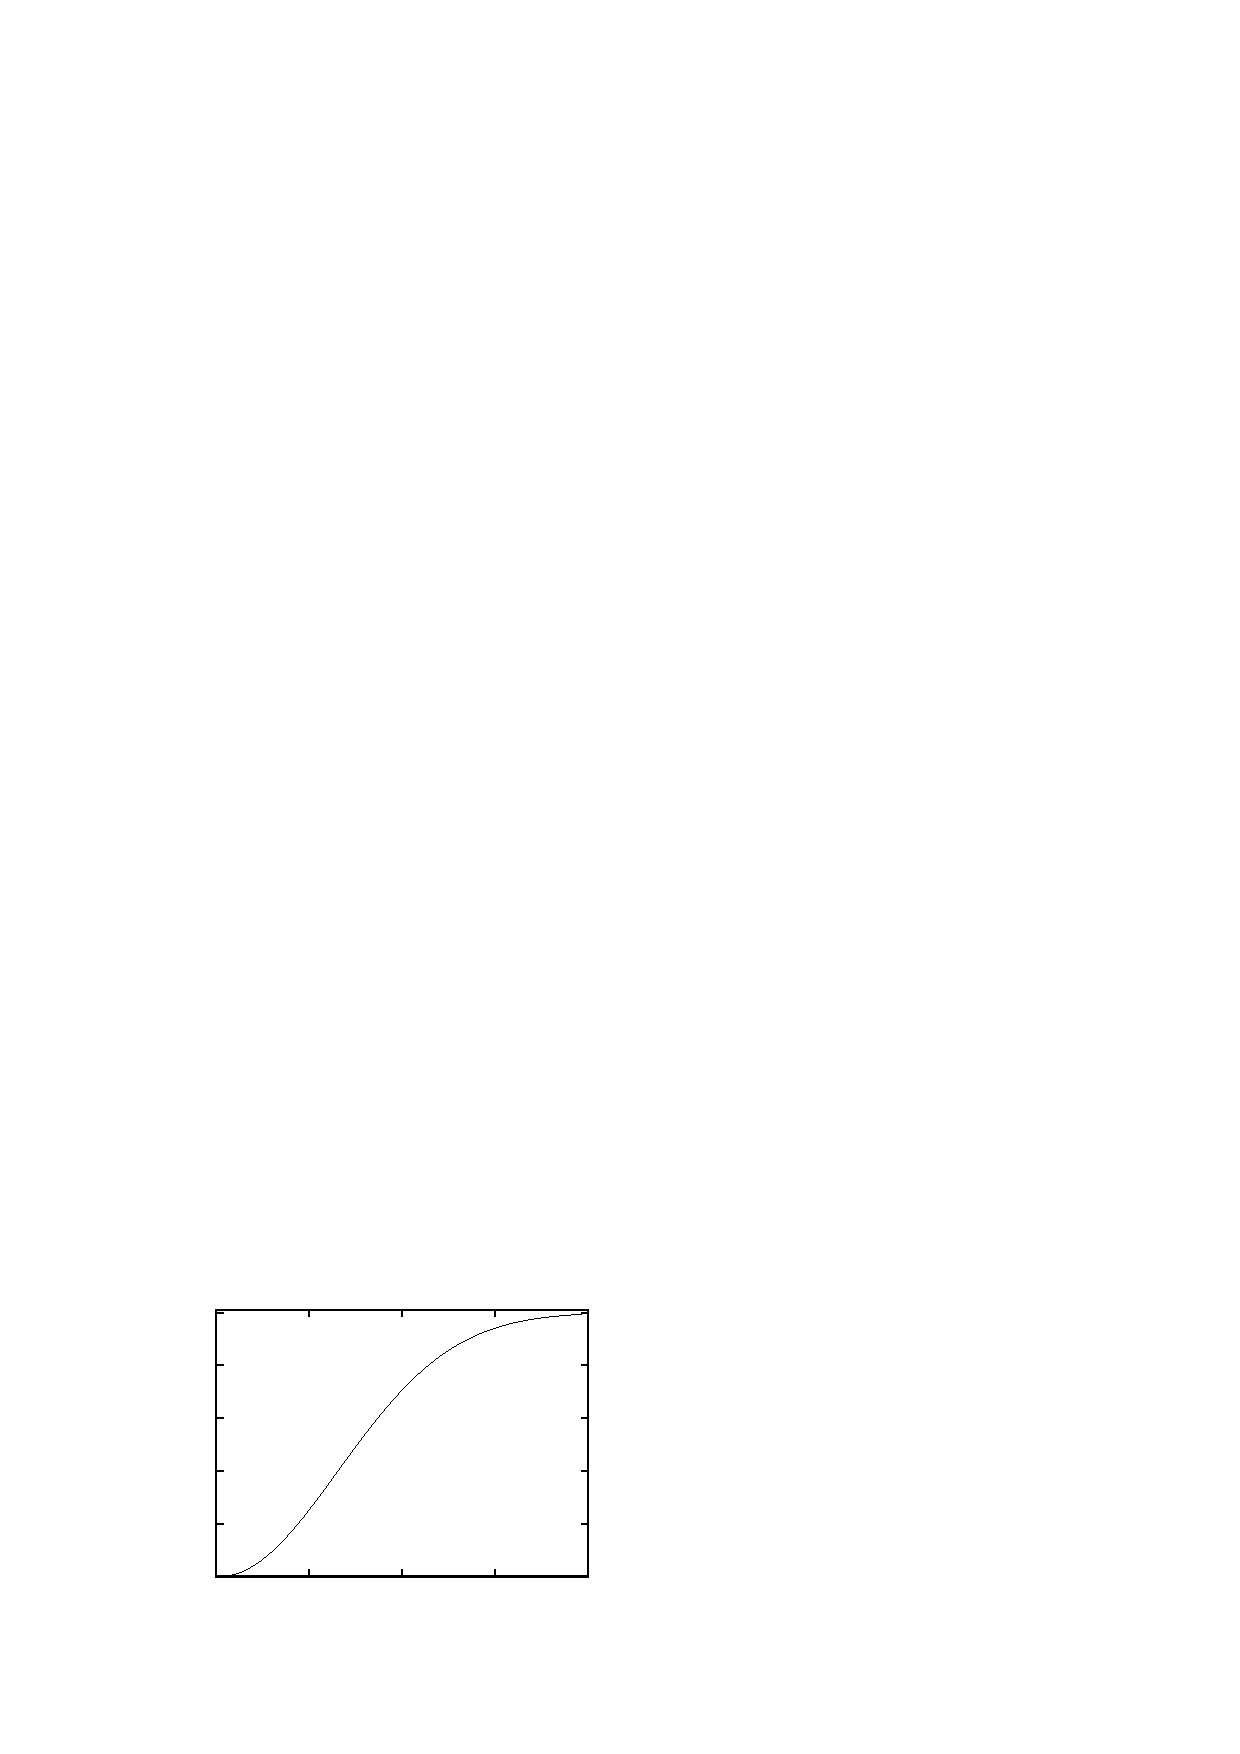
\includegraphics{birthday}}%
    \gplfronttext
  \end{picture}%
\endgroup

\end{center}
\caption{The probability of at least two people having the same birthday in a group of people, plotted against the size of the group. The code for making this graph is \texttt{birthday.jl}\label{fig_birthday}}
\end{figure}

When we were defining the binomial coefficient, we used the factorial
$n!$. The factorial also has a counting function, it counts the number
of ways of ordering a set of size $n$. A similar function is the permutation
\begin{equation}
P^n_r=\frac{n!}{(n-r)!}
\end{equation}
This counts the number of ways of selecting $r$ objects from $n$ where
ordering is taken in to account. Say you had 26 lettered tiled, all
different and you made a random word by choosing five lettered tiles one by one at
random and lining them up as you picked them out. The number of possible words would be
\begin{equation}
P^{26}_5=26\times 25\times 25\times 24\times 23=7893600
\end{equation}
Another useful combinatorial function is the partition function
\begin{equation}
\left(\begin{array}{c} n\\n_1,n_2,\ldots,n_r\end{array}\right)=\frac{n!}{n_1!n_2!\ldots n_r!}
\end{equation}
where $n_1+n_2+\ldots+n_r=n$. The partition function counts the number
of ways a set of $n$ objects can be split up into $r$ subgroups of
sizes $n_1$, $n_2$ and so on to $n_r$.

Imagine there are 20 people who are given four different jobs; the best
job, easy work, lots of pay, requires six people, the second,
inferior job requires four and the other two, even worse jobs, require
five each. The people are supposed to be distributed among the jobs
randomly, but the supervisor's four siblings are all given the best
job. How likely is that to be just good fortune for the sibs? Well the
total number of ways of distributing the jobs is
\begin{equation}
\left(\begin{array}{c} 20\\6,4,5,5)\end{array}\right)=\frac{20!}{6!4!5!5!}
\end{equation}
Now, if the supervisor's four siblings are in the first group, there
are 16 labourers left to distribute, with two places left for the first job. This means the number of ways of assigning the jobs so that the supervisor's siblings all get the first job is
\begin{equation}
\left(\begin{array}{c} 16\\2,4,5,5)\end{array}\right)=\frac{16!}{2!4!5!5!}
\end{equation}
Hence, if giving out the jobs was truly done randomly, the chance the supervisor's siblings all got the good job is
\begin{equation}
p=\left.\frac{16!}{2!4!5!5!}\middle/\frac{20!}{6!4!5!5!}\right.=\frac{16!}{20!}\frac{6!}{2!}
=\frac{6\times 5\times 4\times 3}{20\times 19\times 18\times 17}
\approx 0.0031,
\end{equation}
so not very likely.

\end{document}

